% Copyright 2004 by Till Tantau <tantau@users.sourceforge.net>.
%
% In principle, this file can be redistributed and/or modified under
% the terms of the GNU Public License, version 2.
%
% However, this file is supposed to be a template to be modified
% for your own needs. For this reason, if you use this file as a
% template and not specifically distribute it as part of a another
% package/program, I grant the extra permission to freely copy and
% modify this file as you see fit and even to delete this copyright
% notice. 

\documentclass{beamer}

\usepackage{wrapfig}
\usepackage[style=authoryear]{biblatex}

\bibliography{presentref.bib}

% There are many different themes available for Beamer. A comprehensive
% list with examples is given here:
% http://deic.uab.es/~iblanes/beamer_gallery/index_by_theme.html
% You can uncomment the themes below if you would like to use a different
% one:
%\usetheme{AnnArbor}
%\usetheme{Antibes}
%\usetheme{Bergen}
%\usetheme{Berkeley}
%\usetheme{Berlin}
%\usetheme{Boadilla}
%\usetheme{boxes}
\usetheme{CambridgeUS}
%\usetheme{Copenhagen}
%\usetheme{Darmstadt}
%\usetheme{default}
%\usetheme{Frankfurt}
%\usetheme{Goettingen}
%\usetheme{Hannover}
%\usetheme{Ilmenau}
%\usetheme{JuanLesPins}
%\usetheme{Luebeck}
%\usetheme{Madrid}
%\usetheme{Malmoe}
%\usetheme{Marburg}
%\usetheme{Montpellier}
%\usetheme{PaloAlto}
%\usetheme{Pittsburgh}
%\usetheme{Rochester}
%\usetheme{Singapore}
%\usetheme{Szeged}
%\usetheme{Warsaw}

\title{Impacts of Sagebrush Vegetation }

% A subtitle is optional and this may be deleted
\subtitle{in a Desert Climate on the Atmospheric Boundary Layer}

\author{B. Eng, M. Moody, and T. Morrison}

% - Give the names in the same order as the appear in the paper.
% - Use the \inst{?} command only if the authors have different
%   affiliation.

\institute[University of Utah] % (optional, but mostly needed)
{
%  \inst{1}%
  Department of Mechanical Engineering\\
  University of Utah}
%  \and
%  \inst{2}%
%  Department of Theoretical Philosophy\\
%  University of Elsewhere}
% - Use the \inst command only if there are several affiliations.
% - Keep it simple, no one is interested in your street address.

\date{ME EN 7710 Final Project, 2017}
% - Either use conference name or its abbreviation.
% - Not really informative to the audience, more for people (including
%   yourself) who are reading the slides online

%\subject{Theoretical Computer Science}
% This is only inserted into the PDF information catalog. Can be left
% out. 

% If you have a file called "university-logo-filename.xxx", where xxx
% is a graphic format that can be processed by latex or pdflatex,
% resp., then you can add a logo as follows:

% \pgfdeclareimage[height=0.5cm]{university-logo}{university-logo-filename}
% \logo{\pgfuseimage{university-logo}}

% Delete this, if you do not want the table of contents to pop up at
% the beginning of each subsection:
\AtBeginSubsection[]
{
  \begin{frame}<beamer>{Outline}
    \tableofcontents[currentsection,currentsubsection]
  \end{frame}
}

% Let's get started
\begin{document}

\begin{frame}
  \titlepage
\end{frame}

\begin{frame}{Outline}
  \tableofcontents
  % You might wish to add the option [pausesections]
\end{frame}

% Section and subsections will appear in the presentation overview
% and table of contents.

%%%%%%%%%%%%%%%%%%%%%%% Byron presents intro & part 1 %%%%%%%%%%%%%%%%%%%%%%%%

\section{Introduction}

\subsection{Motivation}
\begin{frame}{Motivation}


	\begin{itemize}
	\item {Benefits of understanding turbulence}
		\begin{itemize}
		\item {NWP}
		\item {Industry}
		\item {Aviation}
		\end{itemize}
	\item {Modelling turbulence}
		\begin{itemize}
		\item {Turbulence is random -- difficult to model}
		\item {More difficult around complex terrain \& vegetation}
		\item {Current methods inaccurate in some environments}
		\end{itemize}
	\end{itemize}
	\begin{figure}
		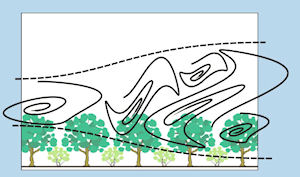
\includegraphics[scale=.3]{pictures/canopy.jpg}
\\ \tiny{\textit{Image source: http://www.windlab.com/technology/turbulence}}
	\end{figure}


\end{frame}

\subsection{MATERHORN Data}

\begin{frame}{MATERHORN}{Overview}
  \begin{itemize}
  \item {MATERHORN Goals:}
  	\begin{itemize}
  	\item {Study limitations of current models in complex terrain}
  	\item {Improve prediction methods}
  	\end{itemize}
  \end{itemize}
  \begin{figure}
  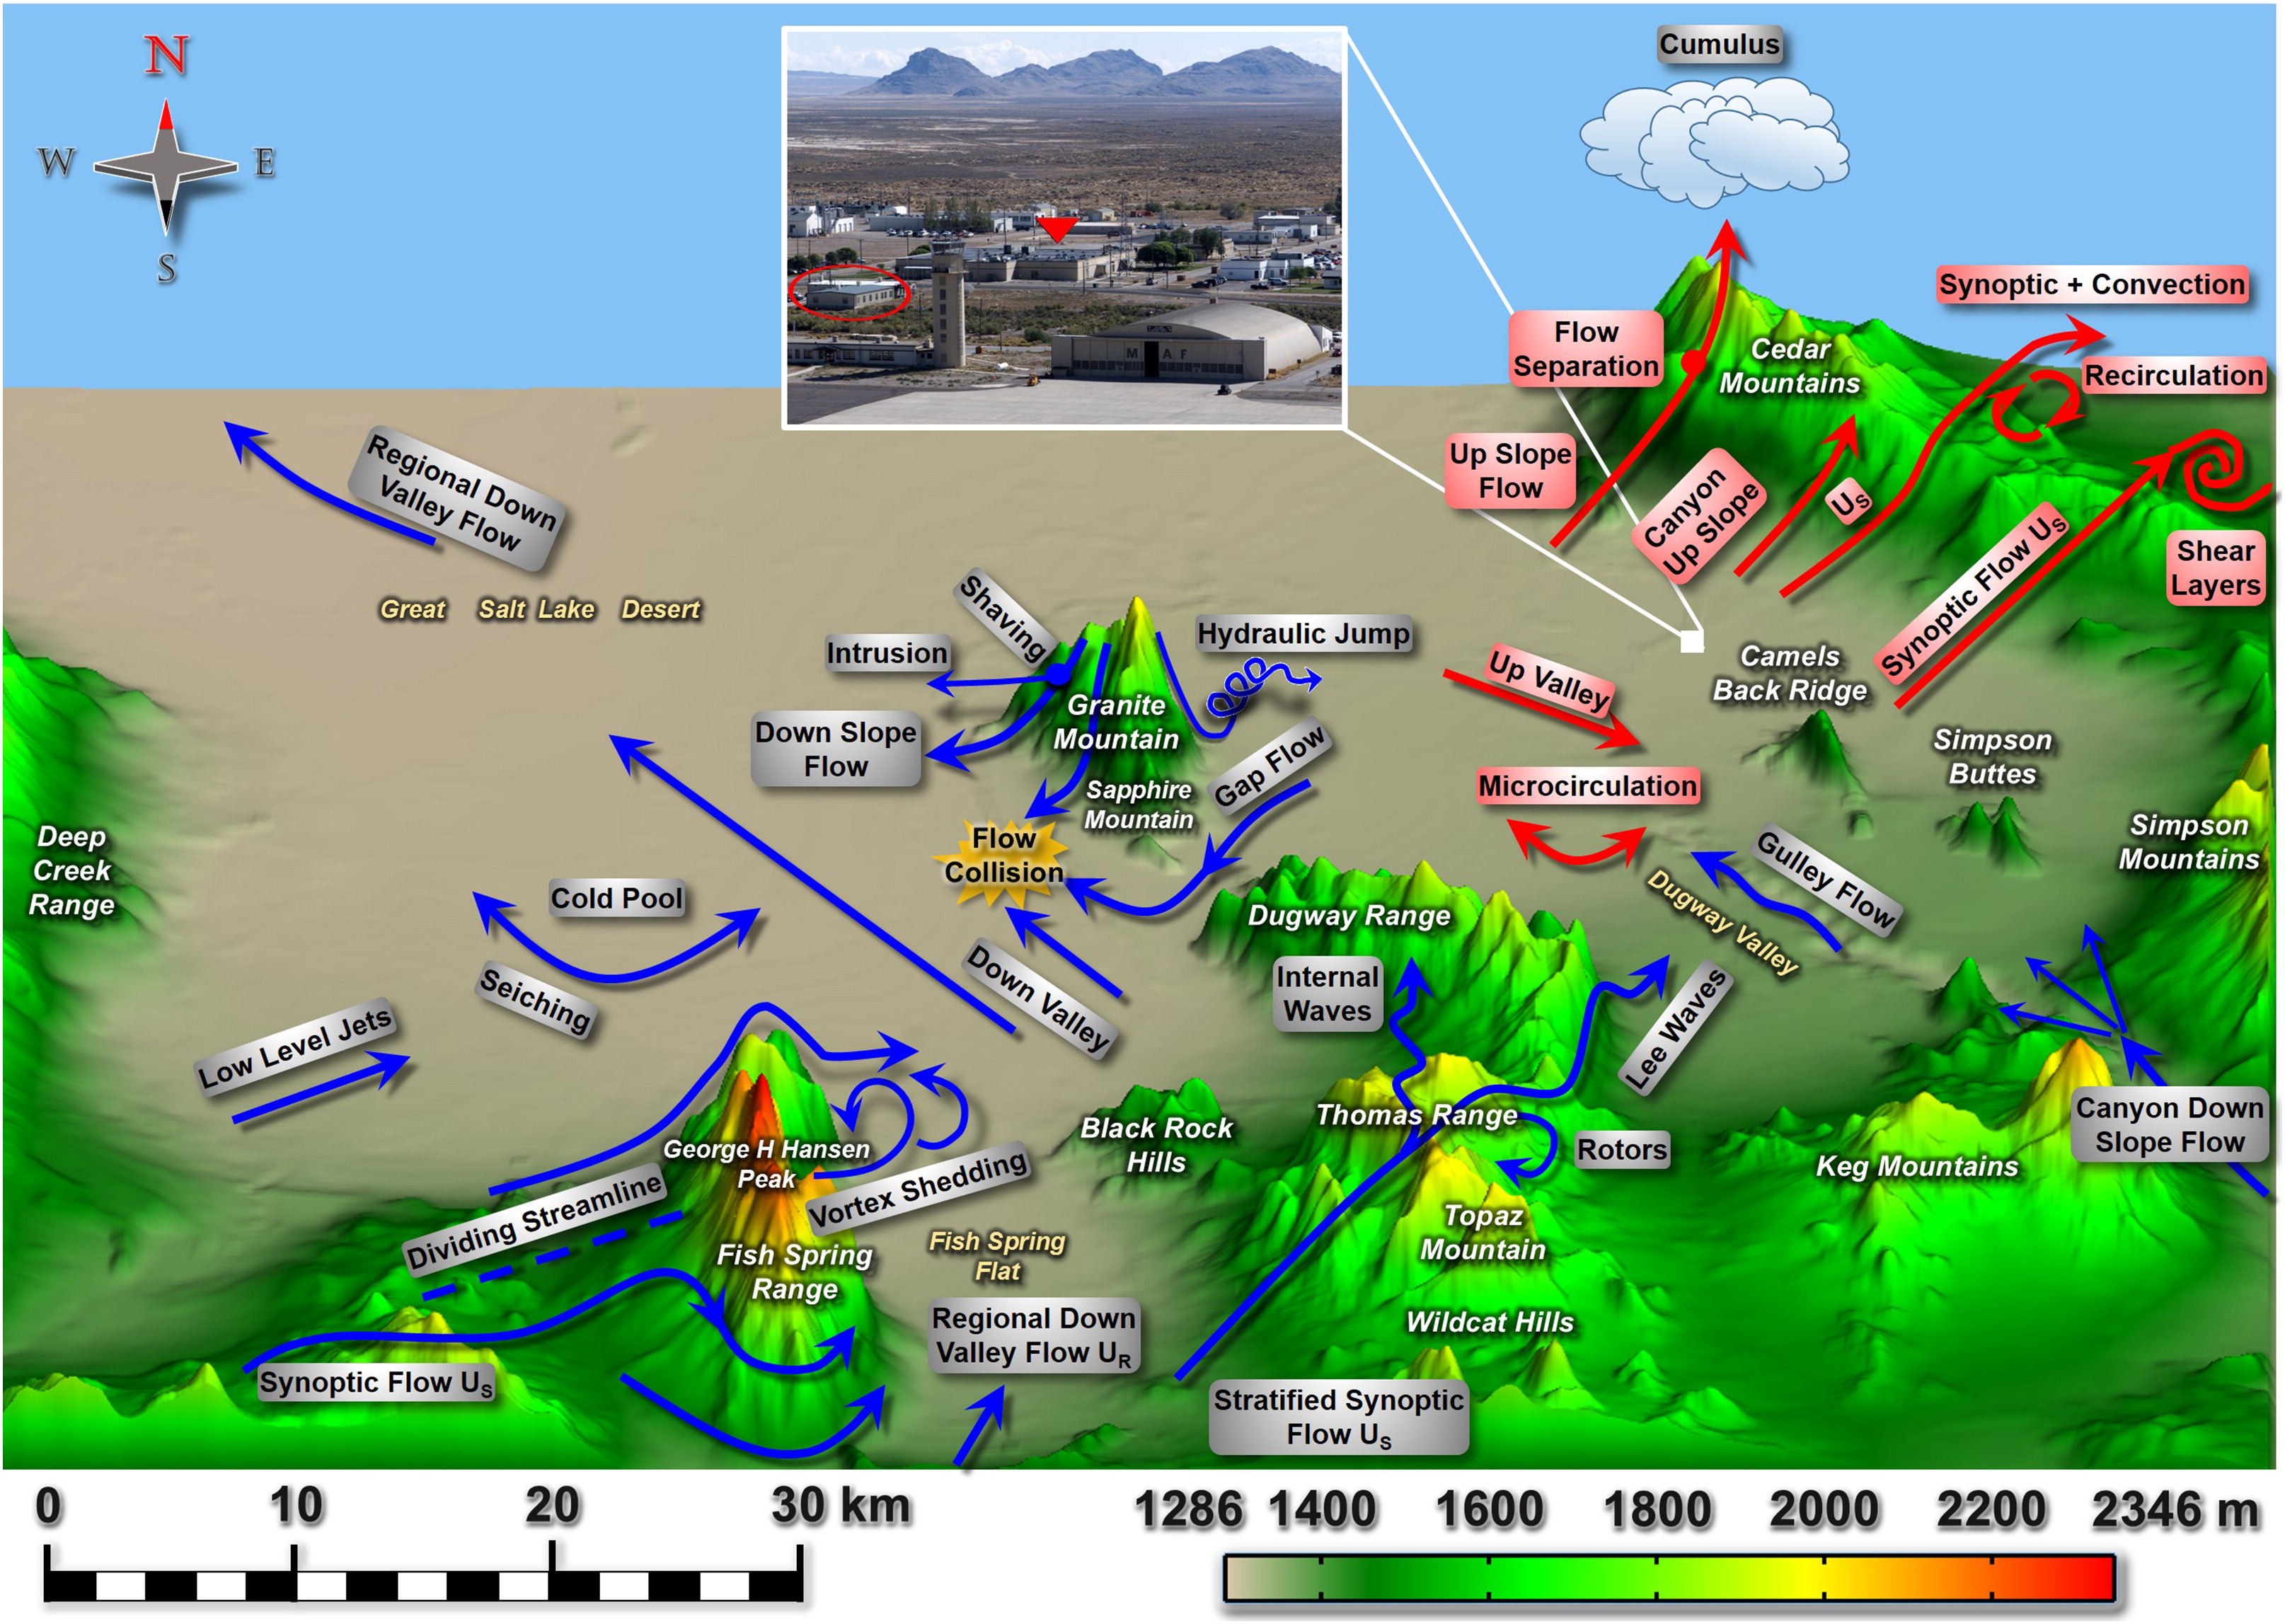
\includegraphics[scale=.4]{pictures/complex.jpeg}
\\  \tiny{\textit{\cite{MATERHORN}}} %I don't know why the citations are messed up
  \end{figure}
  \end{frame}



%\subsection{sample text}
%
%% You can reveal the parts of a slide one at a time
%% with the \pause command:
%\begin{frame}{Second Slide Title}
%  \begin{itemize}
%  \item {
%    First item.
%    \pause % The slide will pause after showing the first item
%  }
%  \item {   
%    Second item.
%  }
%  % You can also specify when the content should appear
%  % by using <n->:
%  \item<3-> {
%    Third item.
%  }
%  \item<4-> {
%    Fourth item.
%  }
%  % or you can use the \uncover command to reveal general
%  % content (not just \items):
%  \item<5-> {
%    Fifth item. \uncover<6->{Extra text in the fifth item.}
%  }
%  \end{itemize}
%\end{frame}

%%%%%%%%%%%%%%%%%%%%%% Travis presents his stuff %%%%%%%%%%%%%%%%%%%%%%%%%
\section{Analysis}

\subsection{Probability Distributions}

\begin{frame}{Blocks}
\begin{block}{Block Title}
You can also highlight sections of your presentation in a block, with it's own title
\end{block}
\begin{theorem}
There are separate environments for theorems, examples, definitions and proofs.
\end{theorem}
\begin{example}
Here is an example of an example block.
\end{example}
\end{frame}

\subsection{Autocorrelation}
\begin{frame}{Autocorrelation}

\end{frame}

%%%%%%%%%%%%%%%%%%%%%% Matt Presents his stuff %%%%%%%%%%%%%%%%%%%%%%%%%%%%

\subsection{Dissipation}
\begin{frame}{Dissipation}

\end{frame}

\subsection{Turbulence Spectra}
\begin{frame}{Turbulence Spectra}

\end{frame}




% Placing a * after \section means it will not show in the
% outline or table of contents.
\section*{Summary}

\begin{frame}{Summary}
  \begin{itemize}
  \item
    The \alert{first main message} of your talk in one or two lines.
  \item
    The \alert{second main message} of your talk in one or two lines.
  \item
    Perhaps a \alert{third message}, but not more than that.
  \end{itemize}
  
  \begin{itemize}
  \item
    Outlook
    \begin{itemize}
    \item
      Something you haven't solved.
    \item
      Something else you haven't solved.
    \end{itemize}
  \end{itemize}
\end{frame}



% All of the following is optional and typically not needed. 
\appendix
\section<presentation>*{\appendixname}
\subsection<presentation>*{For Further Reading}

\begin{frame}[allowframebreaks]
  \frametitle<presentation>{For Further Reading}
    
  \begin{thebibliography}{10}
    
  \beamertemplatebookbibitems
  % Start with overview books.

  \bibitem{Author1990}
    A.~Author.
    \newblock {\em Handbook of Everything}.
    \newblock Some Press, 1990.
 
    
  \beamertemplatearticlebibitems
  % Followed by interesting articles. Keep the list short. 

  \bibitem{Someone2000}
    S.~Someone.
    \newblock On this and that.
    \newblock {\em Journal of This and That}, 2(1):50--100,
    2000.
  \end{thebibliography}
\end{frame}

\end{document}


